%%
%% Automatically generated file from DocOnce source
%% (https://github.com/doconce/doconce/)
%% doconce format html slides3.do.txt SLIDE_TYPE=beamer SLIDE_THEME=red_plain --latex_title_layout=beamer
%%
% #ifdef PTEX2TEX_EXPLANATION
%%
%% The file follows the ptex2tex extended LaTeX format, see
%% ptex2tex: https://code.google.com/p/ptex2tex/
%%
%% Run
%%      ptex2tex myfile
%% or
%%      doconce ptex2tex myfile
%%
%% to turn myfile.p.tex into an ordinary LaTeX file myfile.tex.
%% (The ptex2tex program: https://code.google.com/p/ptex2tex)
%% Many preprocess options can be added to ptex2tex or doconce ptex2tex
%%
%%      ptex2tex -DMINTED myfile
%%      doconce ptex2tex myfile envir=minted
%%
%% ptex2tex will typeset code environments according to a global or local
%% .ptex2tex.cfg configure file. doconce ptex2tex will typeset code
%% according to options on the command line (just type doconce ptex2tex to
%% see examples). If doconce ptex2tex has envir=minted, it enables the
%% minted style without needing -DMINTED.
% #endif

% #define PREAMBLE

% #ifdef PREAMBLE
%-------------------- begin preamble ----------------------

\documentclass[%
oneside,                 % oneside: electronic viewing, twoside: printing
final,                   % draft: marks overfull hboxes, figures with paths
10pt]{article}

\listfiles               %  print all files needed to compile this document

\usepackage{relsize,makeidx,color,setspace,amsmath,amsfonts,amssymb}
\usepackage[table]{xcolor}
\usepackage{bm,ltablex,microtype}

\usepackage[pdftex]{graphicx}

\usepackage{ptex2tex}
% #ifdef MINTED
\usepackage{minted}
\usemintedstyle{default}
% #endif

\usepackage[T1]{fontenc}
%\usepackage[latin1]{inputenc}
\usepackage{ucs}
\usepackage[utf8x]{inputenc}

\usepackage{lmodern}         % Latin Modern fonts derived from Computer Modern

% Hyperlinks in PDF:
\definecolor{linkcolor}{rgb}{0,0,0.4}
\usepackage{hyperref}
\hypersetup{
    breaklinks=true,
    colorlinks=true,
    linkcolor=linkcolor,
    urlcolor=linkcolor,
    citecolor=black,
    filecolor=black,
    %filecolor=blue,
    pdfmenubar=true,
    pdftoolbar=true,
    bookmarksdepth=3   % Uncomment (and tweak) for PDF bookmarks with more levels than the TOC
    }
%\hyperbaseurl{}   % hyperlinks are relative to this root

\setcounter{tocdepth}{2}  % levels in table of contents

% Tricks for having figures close to where they are defined:
% 1. define less restrictive rules for where to put figures
\setcounter{topnumber}{2}
\setcounter{bottomnumber}{2}
\setcounter{totalnumber}{4}
\renewcommand{\topfraction}{0.95}
\renewcommand{\bottomfraction}{0.95}
\renewcommand{\textfraction}{0}
\renewcommand{\floatpagefraction}{0.75}
% floatpagefraction must always be less than topfraction!
% 2. ensure all figures are flushed before next section
\usepackage[section]{placeins}
% 3. enable begin{figure}[H] (often leads to ugly pagebreaks)
%\usepackage{float}\restylefloat{figure}

\usepackage[framemethod=TikZ]{mdframed}

% --- begin definitions of admonition environments ---

% Admonition style "mdfbox" is an oval colored box based on mdframed
% "notice" admon
\colorlet{mdfbox_notice_background}{gray!5}
\newmdenv[
  skipabove=15pt,
  skipbelow=15pt,
  outerlinewidth=0,
  backgroundcolor=mdfbox_notice_background,
  linecolor=black,
  linewidth=2pt,       % frame thickness
  frametitlebackgroundcolor=mdfbox_notice_background,
  frametitlerule=true,
  frametitlefont=\normalfont\bfseries,
  shadow=false,        % frame shadow?
  shadowsize=11pt,
  leftmargin=0,
  rightmargin=0,
  roundcorner=5,
  needspace=0pt,
]{notice_mdfboxmdframed}

\newenvironment{notice_mdfboxadmon}[1][]{
\begin{notice_mdfboxmdframed}[frametitle=#1]
}
{
\end{notice_mdfboxmdframed}
}

% Admonition style "mdfbox" is an oval colored box based on mdframed
% "summary" admon
\colorlet{mdfbox_summary_background}{gray!5}
\newmdenv[
  skipabove=15pt,
  skipbelow=15pt,
  outerlinewidth=0,
  backgroundcolor=mdfbox_summary_background,
  linecolor=black,
  linewidth=2pt,       % frame thickness
  frametitlebackgroundcolor=mdfbox_summary_background,
  frametitlerule=true,
  frametitlefont=\normalfont\bfseries,
  shadow=false,        % frame shadow?
  shadowsize=11pt,
  leftmargin=0,
  rightmargin=0,
  roundcorner=5,
  needspace=0pt,
]{summary_mdfboxmdframed}

\newenvironment{summary_mdfboxadmon}[1][]{
\begin{summary_mdfboxmdframed}[frametitle=#1]
}
{
\end{summary_mdfboxmdframed}
}

% Admonition style "mdfbox" is an oval colored box based on mdframed
% "warning" admon
\colorlet{mdfbox_warning_background}{gray!5}
\newmdenv[
  skipabove=15pt,
  skipbelow=15pt,
  outerlinewidth=0,
  backgroundcolor=mdfbox_warning_background,
  linecolor=black,
  linewidth=2pt,       % frame thickness
  frametitlebackgroundcolor=mdfbox_warning_background,
  frametitlerule=true,
  frametitlefont=\normalfont\bfseries,
  shadow=false,        % frame shadow?
  shadowsize=11pt,
  leftmargin=0,
  rightmargin=0,
  roundcorner=5,
  needspace=0pt,
]{warning_mdfboxmdframed}

\newenvironment{warning_mdfboxadmon}[1][]{
\begin{warning_mdfboxmdframed}[frametitle=#1]
}
{
\end{warning_mdfboxmdframed}
}

% Admonition style "mdfbox" is an oval colored box based on mdframed
% "question" admon
\colorlet{mdfbox_question_background}{gray!5}
\newmdenv[
  skipabove=15pt,
  skipbelow=15pt,
  outerlinewidth=0,
  backgroundcolor=mdfbox_question_background,
  linecolor=black,
  linewidth=2pt,       % frame thickness
  frametitlebackgroundcolor=mdfbox_question_background,
  frametitlerule=true,
  frametitlefont=\normalfont\bfseries,
  shadow=false,        % frame shadow?
  shadowsize=11pt,
  leftmargin=0,
  rightmargin=0,
  roundcorner=5,
  needspace=0pt,
]{question_mdfboxmdframed}

\newenvironment{question_mdfboxadmon}[1][]{
\begin{question_mdfboxmdframed}[frametitle=#1]
}
{
\end{question_mdfboxmdframed}
}

% Admonition style "mdfbox" is an oval colored box based on mdframed
% "block" admon
\colorlet{mdfbox_block_background}{gray!5}
\newmdenv[
  skipabove=15pt,
  skipbelow=15pt,
  outerlinewidth=0,
  backgroundcolor=mdfbox_block_background,
  linecolor=black,
  linewidth=2pt,       % frame thickness
  frametitlebackgroundcolor=mdfbox_block_background,
  frametitlerule=true,
  frametitlefont=\normalfont\bfseries,
  shadow=false,        % frame shadow?
  shadowsize=11pt,
  leftmargin=0,
  rightmargin=0,
  roundcorner=5,
  needspace=0pt,
]{block_mdfboxmdframed}

\newenvironment{block_mdfboxadmon}[1][]{
\begin{block_mdfboxmdframed}[frametitle=#1]
}
{
\end{block_mdfboxmdframed}
}

% --- end of definitions of admonition environments ---

% prevent orhpans and widows
\clubpenalty = 10000
\widowpenalty = 10000

% --- end of standard preamble for documents ---


% insert custom LaTeX commands...

\raggedbottom
\makeindex

%-------------------- end preamble ----------------------

\begin{document}

% matching end for #ifdef PREAMBLE
% #endif

\newcommand{\exercisesection}[1]{\subsection*{#1}}

\input{newcommands_bfmath}
\input{newcommands_replace}

% ------------------- main content ----------------------



% ----------------- title -------------------------

\title{On Schemes for Exponential Decay}

% ----------------- author(s) -------------------------

\author{Hans Petter Langtangen\inst{1,2}}
\institute{Center for Biomedical Computing, Simula Research Laboratory\inst{1}
\and
Department of Informatics, University of Oslo\inst{2}}
% ----------------- end author(s) -------------------------

\date{Jan 32, 2100
% <optional titlepage figure>
% <optional copyright>
}

\vspace{6mm}

% inline figure
\centerline{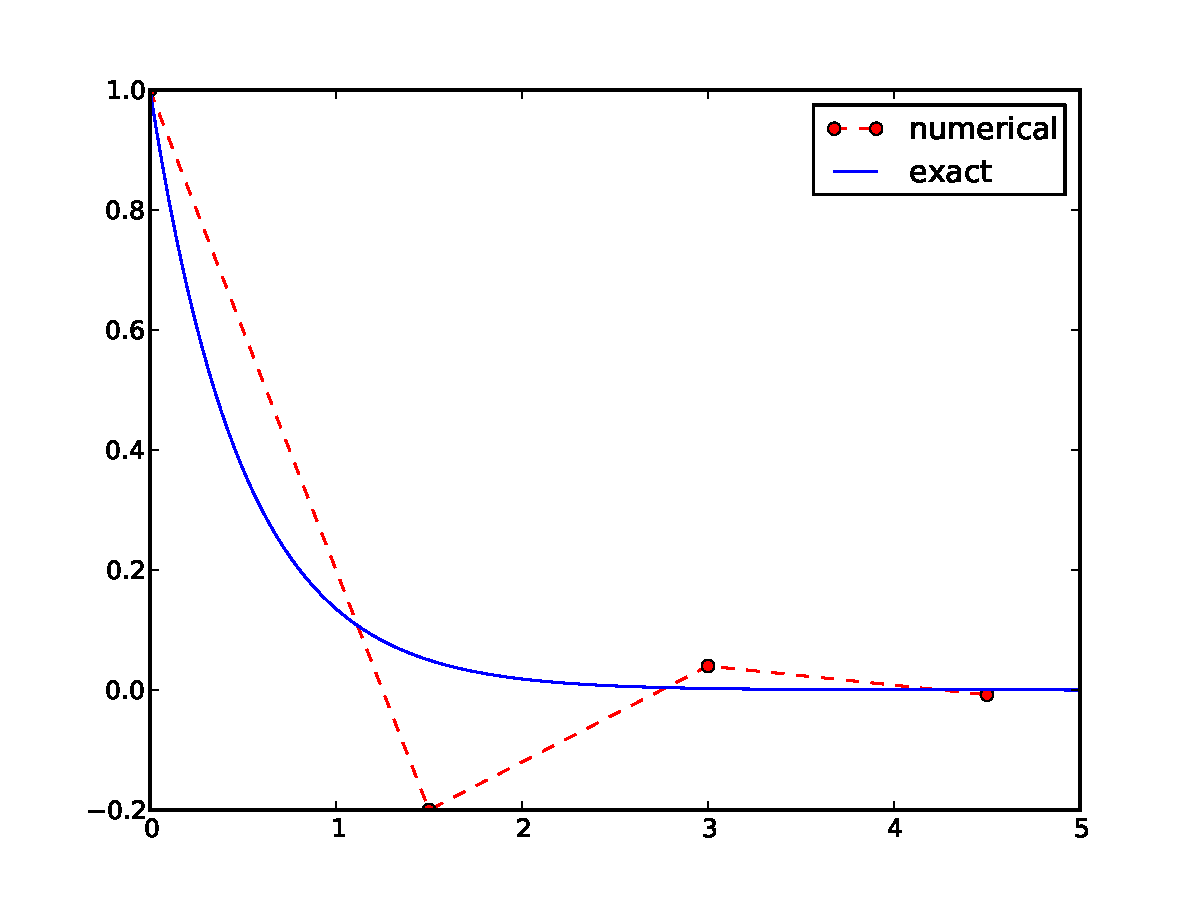
\includegraphics[width=0.4\linewidth]{../doc/src/slides/fig/CN_logo.pdf}}

\vspace{6mm}

% !split
\subsection{Goal}

The primary goal of this demo talk is to demonstrate how to write
talks with \href{{https://github.com/doconce/doconce}}{DocOnce}
and get them rendered in numerous HTML formats.
\begin{block}{Layout }
This version
utilizes beamer slides with the theme red_plain.
\end{block}

% !bnotes
The talk investigates the accuracy of three finite difference
schemes for the ordinary differential equation $u'=-au$ with the
aid of numerical experiments. Numerical artifacts are in particular
demonstrated.
% !enotes

% !split
\section{Methods}

% !split
\subsection{Mathematical problem}

% !bslidecell 00

\begin{align}
u'(t) &= -au(t),
\label{ode}\\ 
u(0)  &= I,
\label{initial:value}
\end{align}

\begin{itemize}
 \item $t\in (0,T]$

 \item $a$, $I$, and $T$ are prescribed parameters

 \item $u(t)$ is the unknown function
\end{itemize}

\noindent
% !eslidecell

% !bslidecell 01

\vspace{6mm}

% inline figure
\centerline{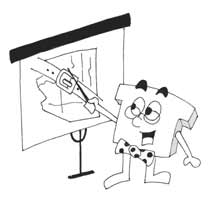
\includegraphics[width=0.5\linewidth]{../doc/src/slides/fig/teacher2.jpg}}

\vspace{6mm}

% !eslidecell

% !split
\subsection{Numerical solution method}

% !bpop
\begin{itemize}
 \item Mesh in time: $0= t_0< t_1 \cdots < t_N=T$

 \item Assume constant $\Delta t = t_{n}-t_{n-1}$

 \item $u^n$: numerical approx to the exact solution at $t_n$
\end{itemize}

\noindent
% !epop

% !bpop
Numerical scheme:
   \[
   u^{n+1} = \frac{1 - (1-\theta) a\Delta t}{1 + \theta a\Delta t}u^n,
   \quad n=0,1,\ldots,N-1
   \]
% !epop

% !split

\subsection{Implementation}

The numerical method is implemented in a Python function:














\bpycod
def solver(I, a, T, dt, theta):
    """Solve u'=-a*u, u(0)=I, for t in (0,T]; step: dt."""
    dt = float(dt)           # avoid integer division
    N = int(round(old_div(T,dt)))     # no of time intervals
    T = N*dt                 # adjust T to fit time step dt
    u = zeros(N+1)           # array of u[n] values
    t = linspace(0, T, N+1)  # time mesh

    u[0] = I                 # assign initial condition
    for n in range(0, N):    # n=0,1,...,N-1
        u[n+1] = (1 - (1-theta)*a*dt)/(1 + theta*dt*a)*u[n]
    return u, t

\epycod


% !split
\section{Selected results}
% Short title: Results

% !split
\subsection{The Crank-Nicolson method}

\vspace{6mm}

% inline figure
\centerline{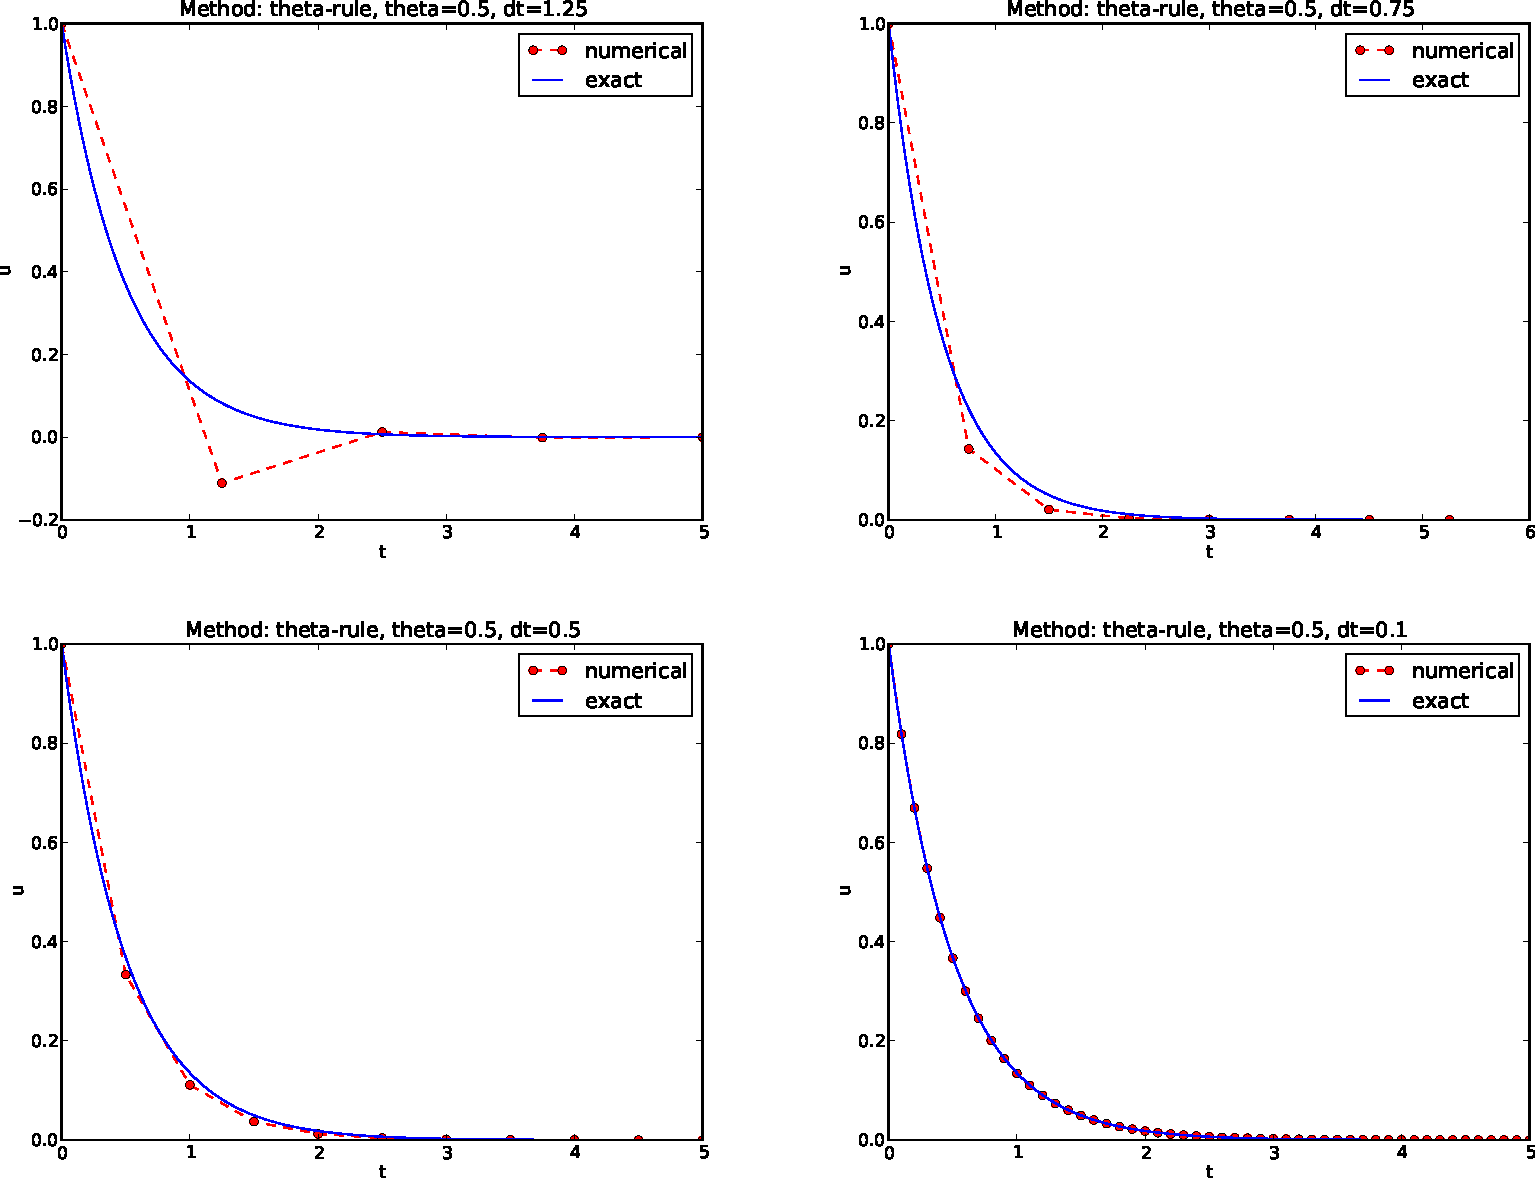
\includegraphics[width=0.9\linewidth]{../doc/src/slides/fig/CN.pdf}}

\vspace{6mm}

% !split
\subsection{The artifacts can be explained by some theory}

% !bpop
Exact solution of the scheme:

\[ u^n = A^n,\quad A = \frac{1 - (1-\theta) a\Delta t}{1 + \theta a\Delta t}\thinspace .\]
% !epop

% !bpop
\begin{itemize}
 \item Stability: $|A| < 1$

 \item No oscillations: $A>0$

 \item Always for Backward Euler ($\theta=1$)

 \item $\Delta t < 1/a$ for Forward Euler ($\theta=0$)

 \item $\Delta t < 2/a$ for Crank-Nicolson ($\theta=1/2$)
\end{itemize}

\noindent
% !epop

% !bpop
\begin{block}{Concluding remarks: }
Only the Backward Euler scheme is guaranteed to always give
qualitatively correct results.
\end{block}
% !epop

% ------------------- end of main content ---------------

% #ifdef PREAMBLE
\end{document}
% #endif

